\section{Introduction}
\label{S:TInt}

The rapid technological development in Automated Vehicles (AVs), followed by a tremendous increase in their adoption, promises a significant transformation in the dynamics on urban roads. An important transformation expected to occur is the effect of AVs on pedestrians, as the most vulnerable road users. Particularly, in the absence of a driver in the vehicles, and thus the absence of eye contact and observation and interpretation of head and body movements by the driver, the interaction between vehicle and pedestrian has to be re-investigated to account for the resulting changes. To be able to compensate for the silent agreement between the driver and pedestrian, and establish a similar type of interactions between pedestrians and vehicles in an automated environment, AVs need to find a way to anticipate pedestrian behaviour, i.e. intentions, choices and movements/trajectories, based on the pedestrian reactions captured. Failures in the prediction of pedestrian behaviour and the absence of timely actions by the AV have already resulted in catastrophic accidents in recent years, even at very slow speeds~\citep{uber,vienna}.

Studying pedestrian behaviour is an active and extensive area of research. In this study, however, we focus on behaviour of pedestrians when crossing mid-block, unsignalized roads. As rule-obeying AVs find their way on the streets in future urban spaces, it is a plausible scenario that this type of crossing increase in spatio-temporal frequency~\citep{millard2018pedestrians}. Going through the official reports of uber's test AV incidence in Arizona, it appeared that the vehicle's system could not predict the pedestrian's path correctly because she was crossing mid-block, and \textit{"the system design did not include consideration for jaywalking pedestrians."}~\citep{uber,ntsb}. Thus, a thorough investigation of mid-block crossings is timely and of vital importance. 

We can simplify the interactions of an AV and a pedestrian crossing mid-block to three parts~\cite{kalatian2020decoding}. As depicted in \cref{fig:Tinteraction}, (a) a pedestrian waits on the sidewalk for the right time to initiate a cross, (b) They then follow a certain trajectory based on the characteristics of the approaching vehicle, and geometric and environmental conditions. On the other hand, the vehicle anticipates pedestrian behaviour and reacts to it by making the required decisions to provide a safe and comfortable crossing for the pedestrian while accounting for the passengers' safety and comfort. We explored the first part of this interaction, i.e., wait time of pedestrian, in two previous studies~\cite{kalatian2019deepwait,kalatian2020decoding}. Here the focus is to understand and develop prediction models for the second part, the pedestrian trajectory. Together, the two behaviour prediction models can then be used by AVs to anticipate pedestrian movement better and proactively make maneuvering decisions~\cite{vasquez2019multi}.

\begin{figure}
    \centering
    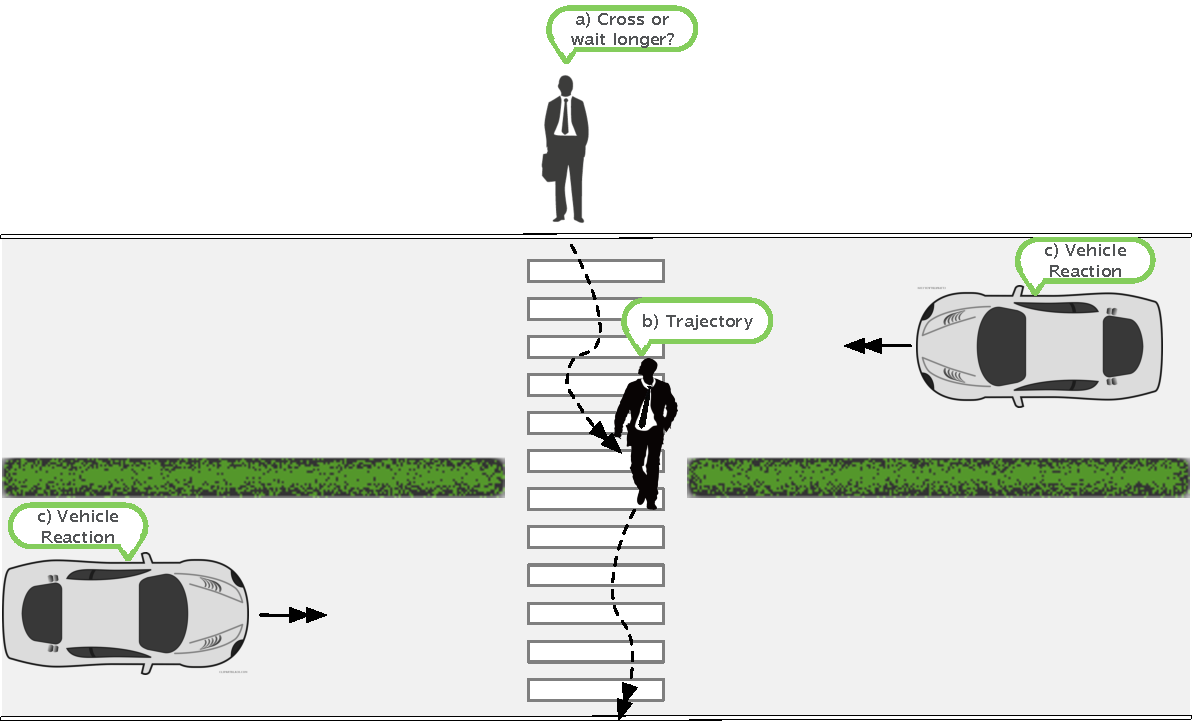
\includegraphics[scale=0.7]{chapter_6/figures/cross.pdf}
    \caption{Schematic representation of vehicles and pedestrians interactions}
    \label{fig:Tinteraction}
\end{figure}

Given an initial observation of the behaviour, as well as contextual information of the environment in which the crossing takes place, we developed a prediction model to estimate the trajectory of a pedestrian. By providing an extensive review of the open-access AV datasets, we discuss existing gaps within them. Data used to train and test the models in this study are collected using the Virtual Immersive Reality Environment (VIRE)~\cite{farooqvire} framework. Virtual Reality (VR) tools have made it possible to create an immersive and controlled environment in which detailed pedestrian behaviour can be analyzed under specific sets of conditions.. 

A novel multi-input network of Long Short-Term Memory (LSTM) and fully connected dense layers is developed to model trajectories of pedestrians while they cross a road in an automated environment. In the proposed model, time-series data of the initial steps of crossing, including trajectories, head orientations, and distance to vehicles, are added to non-time-series data of contextual information of the crossing's environment to predict the next steps of pedestrian trajectories. A game theory-based post-hoc interpretability method for neural networks is applied to analyze the contributing factors to pedestrian trajectory prediction. By providing insights into the most determining factors in trajectory prediction, we propose suggestions that can help to improve currently available datasets from a pedestrian-oriented point-of-view.  

The rest of this paper is organized as follows: a review of relevant studies in trajectory prediction and an extensive review of currently available open-access AV datasets are provided in the next section. \cref{S:t3} briefly discusses data collection and pre-processing procedures. Methodology and proposed architecture are described in \cref{S:t4}. The application of our proposed framework on the data and their interpretation are discussed in \cref{S:t5}. Finally, \cref{S:t6} is dedicated to conclusions, final remarks, and future research plans of the project.